\clearpage
\section{Related Work}
\label{sec:related-work}

The aim of this section is to describe the existing work that has been done on multimodal machine learning to classify road defects. However, to my knowledge, this has never been researched yet. What we did find is research using a single source of data in machine learning pipelines. This section will therefore review what is known in automatic road defects classification. Finally, we look briefly at current literature on multimodal machine learning in general.

% TODO: table with all keywords and search results

% Literature to answer these questions will be gathered with the following procedure:
% \begin{enumerate}
% \item List search relevant search terms.
% \item Find synonyms in a thesaurus.
% \item Search literature on Google Scholar \cite{scholar}, Science Direct \cite{science-direct} and Papers with Code \cite{paperswithcode}. 
% \item Select potential papers based on their title and abstract.
% \item Check Google Scholar which cite the respective paper to see if a more recent version exists (forward citation).
% \item Scan through paper references if a specific title seems relevant (backward citation), repeat from 4.
% \end{enumerate}

From our review we discover that there is whole research field around data driven road defects classification. Motivations for research is that the conventional way of assessing the road quality is perceived as: expensive, labor-intensive, and requires (subjective) domain expertise. As mentioned earlier, there is already a lot of types of data collected to assess the road quality. This is typically done with a specialized vehicle (see \ref{fig:aran-vehicle}). As this vehicle is expensive, it is difficult to apply on large scale. Researchers therefore focus on alternative forms to collect the data with cheaper methods. Smartphones are for instance often used as they already contain a camera and accelerometer. In literature identified we the following fields researching road quality based on the used data: ``visual surface defects'' uses camera based sensors, ``sensor surface defects'' and ``roughness evaluation'' uses the accelerometer, and ``noise labelling'' uses an external microphone.

\begin{figure}[h!]
\begin{center}
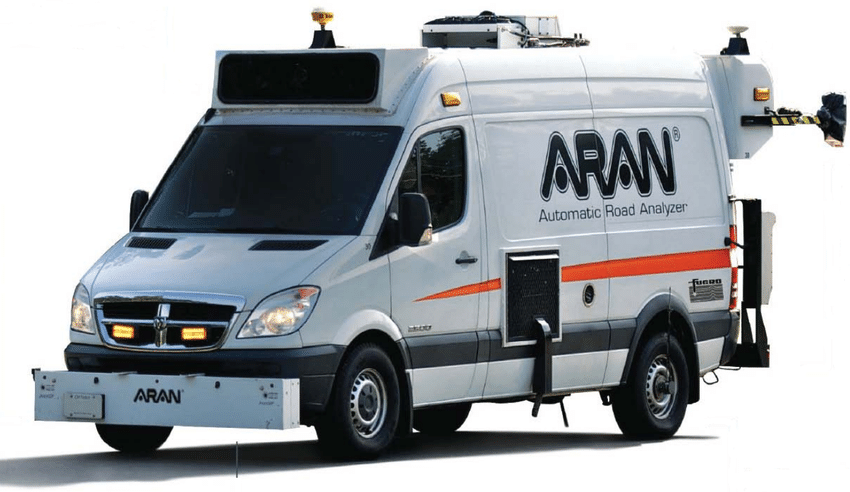
\includegraphics[height=5cm,keepaspectratio]{images/2_literature/aran.png}
\end{center}
\caption{Automatic Road Analyzer (ARAN) is specialized vehicle to gather data about the road surface \cite{Gupta2020}.}
\label{fig:aran-vehicle}
\end{figure}

\subsection{Visual Surface Defects}
\label{sec:visual-surface-defects}

Visual surface defects are based on visual techniques to automatically classify damages. Especially more recently smartphones are used. However, researchers have also used dashcams, and Microsoft Kinect. Kinect is equipped with a RGB camera, and an infrared camera to measure depth. In \authorref{Jahanshahi2012} the authors uses a Kinect sensor to collect image and depth data. Recording of the road has been performed from a top-faced perspective. The authors classify cracks, potholes and patches with accuracy scores of respectively 78\%, 92\% and 90\%. By including depth information, the problem of detecting defects is relatively trivial. Classifying defects is done by checking if the depth is greater than some threshold.

In 2016, the first model was published using machine learning to detect road cracks by \authorref{Zhang2016}. The data is collected by smartphones from a top-faced perspective of known defects. Their research objective is to train a deep convolutional neural network to classify if a specific image patch is a damage or not. Related to this work is \authorref{Zhang2017}, the authors use 3D pavement images to classify each pixel in a patch individually as crack or no crack. Their objective is focused on acquiring pixel-level accuracy. This is interesting as it describes the severity of the damage (i.e., the size and location). Both methods are similar in collecting and training a deep convolutional neural network. However, their models are specifically trained on small patches, omitting the actual global context (i.e., the actual road). This means that their models wouldn't generalize well and are hard to deploy in the real world.

One of the earlier methods that collects data in a realistic setting is that of \authorref{Chatterjee2018}. The authors perform road crack detection on cycling roads in Germany. They use a smartphone attached to a bicycle, and record the road surface from a front-faced perspective. The data is then pre-processed using various computer based algorithms. Subsequently, the extracted features are used in different machine learning models to evaluate performance. Although their method works well, it is not a complete end-to-end machine learning pipeline.

The first complete pipeline is performed in \authorref{Maeda2018}. Data was collected from a smartphone in a typical holder attached to the windshield. The authors extensively collect data about Japanese roads. Contributions of their research include their results, but additionally contribute the collected data, and a pre-trained model. The dataset is known as Road Damage Dataset by \authorref{road-damage-detector}, and receives updates the following years. This is also the first research to include multiple types of damages, i.e., fading road markings, and distinction between types of cracks. Instead on focusing on specific image patches, the authors frame the problem as object detection.

The research is extended in \authorref{Arya2020-transfer}, where the authors update the dataset by collecting data from Czech Republic and India. The researchers use transfer learning to evaluate the generalization of the developed model in different countries. They conclude that it is difficult to achieve decent performance when using the model in a different country. Although no explicit reasons are given, this can be expected as different countries build their infrastructure in different ways. However, when the model is transfer learned on images from that respective country, the performance does increase more rapidly, and the yielded model is more generalizable. 

To improve performance, the authors of \authorref{Maeda2020} use a Generative Adverserial Network (GAN) to augment the dataset with more data. This also improves generalizability. With a GAN two neural networks are trained and compete with each other. One model, the generator, tries to generate samples as if they came from the original distribution set. Another model, the discriminator, receives either a real image or a generated sample, and tries to classify if a given sample is real or fake. Overtime, the generator mimics the original distribution, and is capable of generating more samples. With more training data, the model performs better as it is less likely to overfit, and generalizes better. The model is retrained on this augmented dataset, and the authors report a 5\% increase in performance.

Another effort to improve the performance of the model is that a public competition was held {Arya2020-competition}. The aim of the competition was to push the state-of-the-art of detecting road surface defects forward. Current best performance for a single class was F1 score of 0.40. The winner of the competition achieved an average (for all classes) F1 score of 0.67 \cite{rddc2020}. The earlier models \cite{Maeda2018,Arya2020-transfer,Maeda2020} all used Single Shot Detector to detect the damages. Whereas, the winning model was trained on YOLOv5 \cite{Jocher2021}. This model is currently regarded as state-of-the-art in object detection. How object detection works is later described in section \ref{sec:object-detection}.


\subsection{Sensor Surface Defects}
Sensor surface defects use non-visual data sources to classify defects. Most commonly used is the accelerometer. This is a sensor which measures the change in velocity over time. Typically an accelerometer measures in three directions: X, Y and Z. When the vehicle drives over a damage, e.g., a pothole, the car vibrates and these vibrations are measured with an accelerometer. The output is in G-forces, where $1 G = 9.81m/s^2$. In stationary position, the accelerometer always measures 1G on the vertical axis due gravitational pull of the earth.

Detecting potholes using accelerometer of smartphone is often researched. For instance are the works of \authorref{Wu2020} and \authorref{Basavaraju2019}. Both papers use machine learning to detect potholes using smartphones. Interestingly, both works follow similar methodology, consisting of four stages: (1) data acquisition, (2) data processing, (3) feature extraction, and (4) classification. The data is processed into sliding windows. On these windows various signal processing operations are performed, and features are extracted. Detection of damages is subsequently done with different machine learners (e.g., Random Forests, Support Vector Machines).

During the data processing stage, both papers perform the following operations: resampling, reorientation, and filtering. The key data processing operations is the reorientation (or realignment) of the accelerometer with respect to the vehicle. In order to use the data, the coordinate systems of the accelerometer and the vehicle must coincide. For instance, when the vehicle experiences a vertical force, we want that respective force also measured on the vertical axis of the accelerometer. In practice is it is unlikely that the accelerometer in the smartphone is perfectly aligned with that of the car. This problem is also applicable in this work, and the process of reorientation will be discussed in depth later in section \ref{sec:reorientation}. 

There are a few differences in the research of \authorref{Basavaraju2019}. First of all, it performs multi-class detection between cracks, potholes, and smooth roads. Another key difference is that the authors of \authorref{Basavaraju2019} also evaluate an end-to-end pipeline with a neural network. In that experiment, they skip the feature extraction but directly learn from the preprocessed signal. As the authors expected, the performance deteriorated slightly. The main advantage is the time saved on feature extraction. Given enough data, the authors expect that the neural network can perform just as well.


\subsection{Road Roughness (IRI)}
Besides detecting surface defects, accelerometer is also used to estimate the ``road roughness''. Which is defined as ``the deviation of the surface from the true planar surface''. This deviation affects vehicle dynamics and ride quality. Two methods to classify the roughness of a profile are the ``International Roughness Index'' (IRI) \cite{Sayers1986} and the International Standards Organisation (ISO) \cite{ISO8608} classification. 

The conventional method to measure the road's profile is done with an inertial profiler. This is a device which scans the surface of the pavement with lasers to measure the distance between the road and the sensor. This sensor is also equipped on the specialized Automatic Road Analyzer (ARAN) vehicle (see figure \ref{fig:aran-vehicle}). From review, we see that there is a large amount of research focused on estimating IRI using an accelerometer found in smartphones \cite{Hanson2014,Buttlar2014,Gupta2020,Jeong2020}. All researchers followed a similar approach. The accelerations were collected with a smartphone. From the collected data, only data from the vertical axis was extracted. This was subsequently passed through a proprietary tool to calculate the IRI profile. The resulting profile was compared with that of the ground truth, and all research found that smartphones can accurately measure IRI in most cases.


\subsection{Noise Labelling}
The road quality influences the noise and vibrations emission caused by the interaction between tires of the vehicle and the road. Within the EU, member states are obliged to publish noise maps for their infrastructure every five year \cite{EU2002}. These emissions can be recorded with specialized equipment, e.g., a Close Proximity Trailer (CPX). In \authorref{Hauwermeiren2019}, the authors try to replicate the results of CPX measurements by using a sensor box containing a microphone. The microphone is located in the trunk of the car. The authors were able to accurately estimate the road texture. However, this experiment was performed under strict conditions by eliminating background noises (e.g., the radio was turned off, and no talking). The authors continued their research in \authorref{Hauwermeiren2021}, where they use multiple vehicles and non-standard driving conditions. They found that below 1600 Hz, that the gathered results were accurate enough to replace the CPX measurement.

\begin{figure}[ht]
\begin{center}
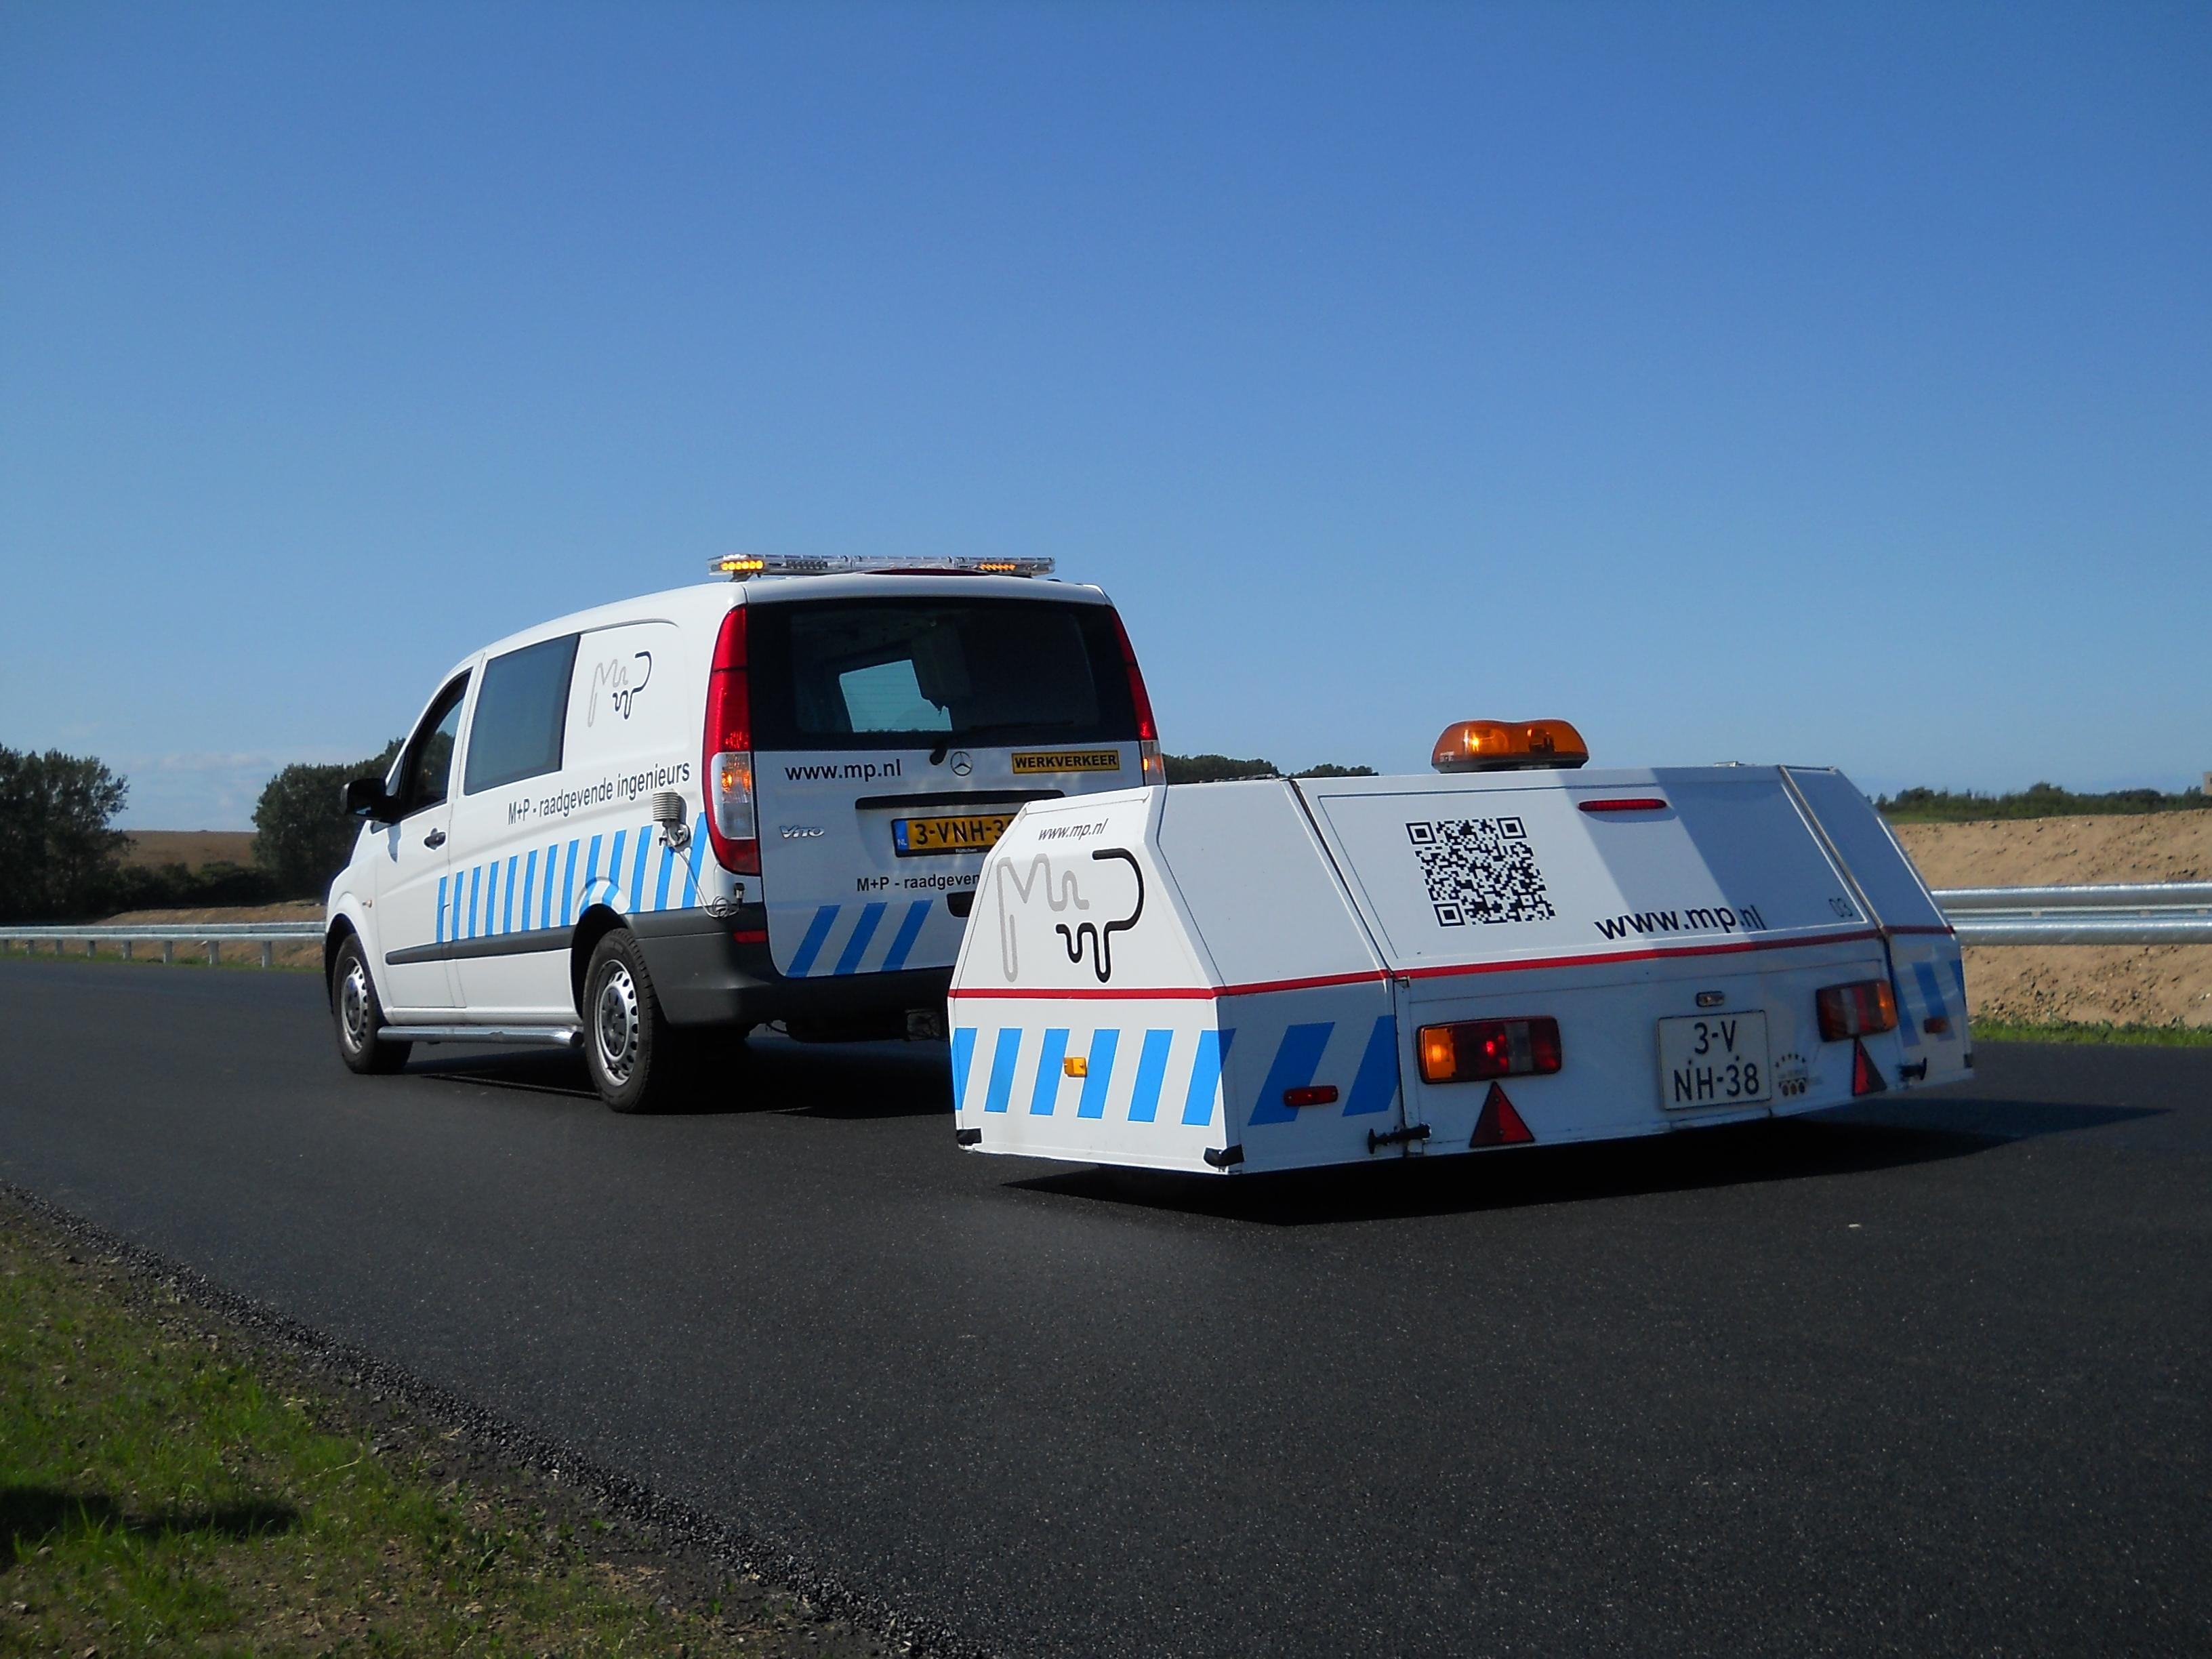
\includegraphics[height=5cm,keepaspectratio]{images/2_literature/cpx-trailer.jpg}
\end{center}
\caption{Close Proximity (CPX) trailer measures the sounds emitted by reference tyre \cite{MP2020}.}
\end{figure}


\subsection{Combination of Visual and Accelerometer}
As previously mentioned there is no current work on combining visual and accelerometer data in a complete end-to-end machine learning pipeline. However, in the paper of \authorref{Lekshmipathy2020}, the researchers compare both methods. Accelerometer data is collected with an smartphone attached to the windshield. Without further processing, the data was fed to a neural network and classified either as: no defect, pothole, patch, crack, or bump. The model was able to distinct the different types of damages with an accuracy of 80 \%. For the visual method, the authors collected image data from a top down view perspective. After applying various image processing operations, the authors use a threshold based method to classify visual surface defects. The resulting model slightly outperforms the vibration based method with accuracy of 84 \%. The authors argue that for continuous monitoring the state vibration based method is sufficient, and resort to the visual method when there is need for higher accuracy.

Another research that uses both data sources is that of \authorref{Lee2021}. Again, the authors don't use both sources simultaneously in an end-to-end pipeline. However, this research is still interesting. The researches use a smartphone to collect both sources of data. This time, the image data is recorded from a front-faced perspective. The researches created a visual model to detect road anomalies, and incorporated it into their collection app. When the app detected an anomaly, the accelerometer data is recorded for three seconds. From this data, they make a comparison between the different type of damages, and the response on the accelerometer. They argue that it is hard with only visual data to measure the severity of an anomaly. By including the accelerometer data classifying the severity becomes easier.



\subsection{Multimodal Machine Learning}
\label{section:multimodal-ml}

We experience the world as multimodal: we see objects, feel vibrations and hear sounds. Modality refers to the way in which something happens or is experienced. A research problem is characterized as multimodal when it includes multiple of such modalities \cite{Baltrusaitis2017}. Commonly referred example of an everyday multimodal experience is the McGurk effect \cite{McGurk1976}. This is the perception between hearing and vision in speech: when we hear the syllable /ba/ while watching the lips of someone saying /ga/, we perceive it as /da/. 

In the work by \authorref{Baltrusaitis2017} multimodal fusion is described as integrating information from multiple modalities with the goal of predicting an outcome. There are three main benefits it can provide. First, having access to multiple modalities that observe the same event allow for better predictions. Second, multiple modalities might complement each other. Third, a multimodal system can still operate when one of the modalities is missing. 

Multimodal research has a long history from audio-visual speech recognition to more recent interest due deep learning \cite{Ngiam2011}. It has been proven that multimodal learning algorithms performs really well on various tasks, such as (audio-visual) speech recognition \cite{Noda2014}, image sentence matching \cite{Ma2015} and RGB-D object recognition \cite{Eitel2015,Xu2017,Sindagi2019}.

\authorref{Baltrusaitis2017} identified five challenges dealing with multimodal machine learning:
\begin{enumerate}
\item \textbf{Representation}: how to represent and summarize multimodal data to exploit the complementary and redundancy of multiple modalities. Distinction is made between \textit{joint representation} - which combines unimodal signals in the same space, and \textit{coordinated representation} - which processes unimodal signals separately, but enforces similarity constraints. See figure \ref{fig:structure-joint-coordinated} below for an illustration.
\item \textbf{Translation}: how to translate data from one modality to another. For example, given an image the task is to give a caption to describe the image.
\item \textbf{Alignment}: how to identify direct relations between (sub)elements from multiple modalities. For example, given an image and a caption, find the area in the image describing the caption.
\item \textbf{Fusion}: how and when to fuse / join information from multiple modalities. Historically the original topics of multimodal machine learning, with emphasize given on early-, hybrid- and late-fusion.
\item \textbf{Co-learning}: how to transfer knowledge between modalities. For example by exploiting knowledge of a rich modality, to aid modelling of a less describing modality.
\end{enumerate}

There are various methods to implement multimodal machine learning. One of these methods is using neural networks. The inputs of the data sources can directly be used as inputs to the neural network. One of the advantages of using neural networks is that it is easy to train an end-to-end model \cite{Ngiam2011,Baltrusaitis2017}. However, the disadvantage is their lack of interpretability. 

\begin{figure}[ht]
\begin{center}
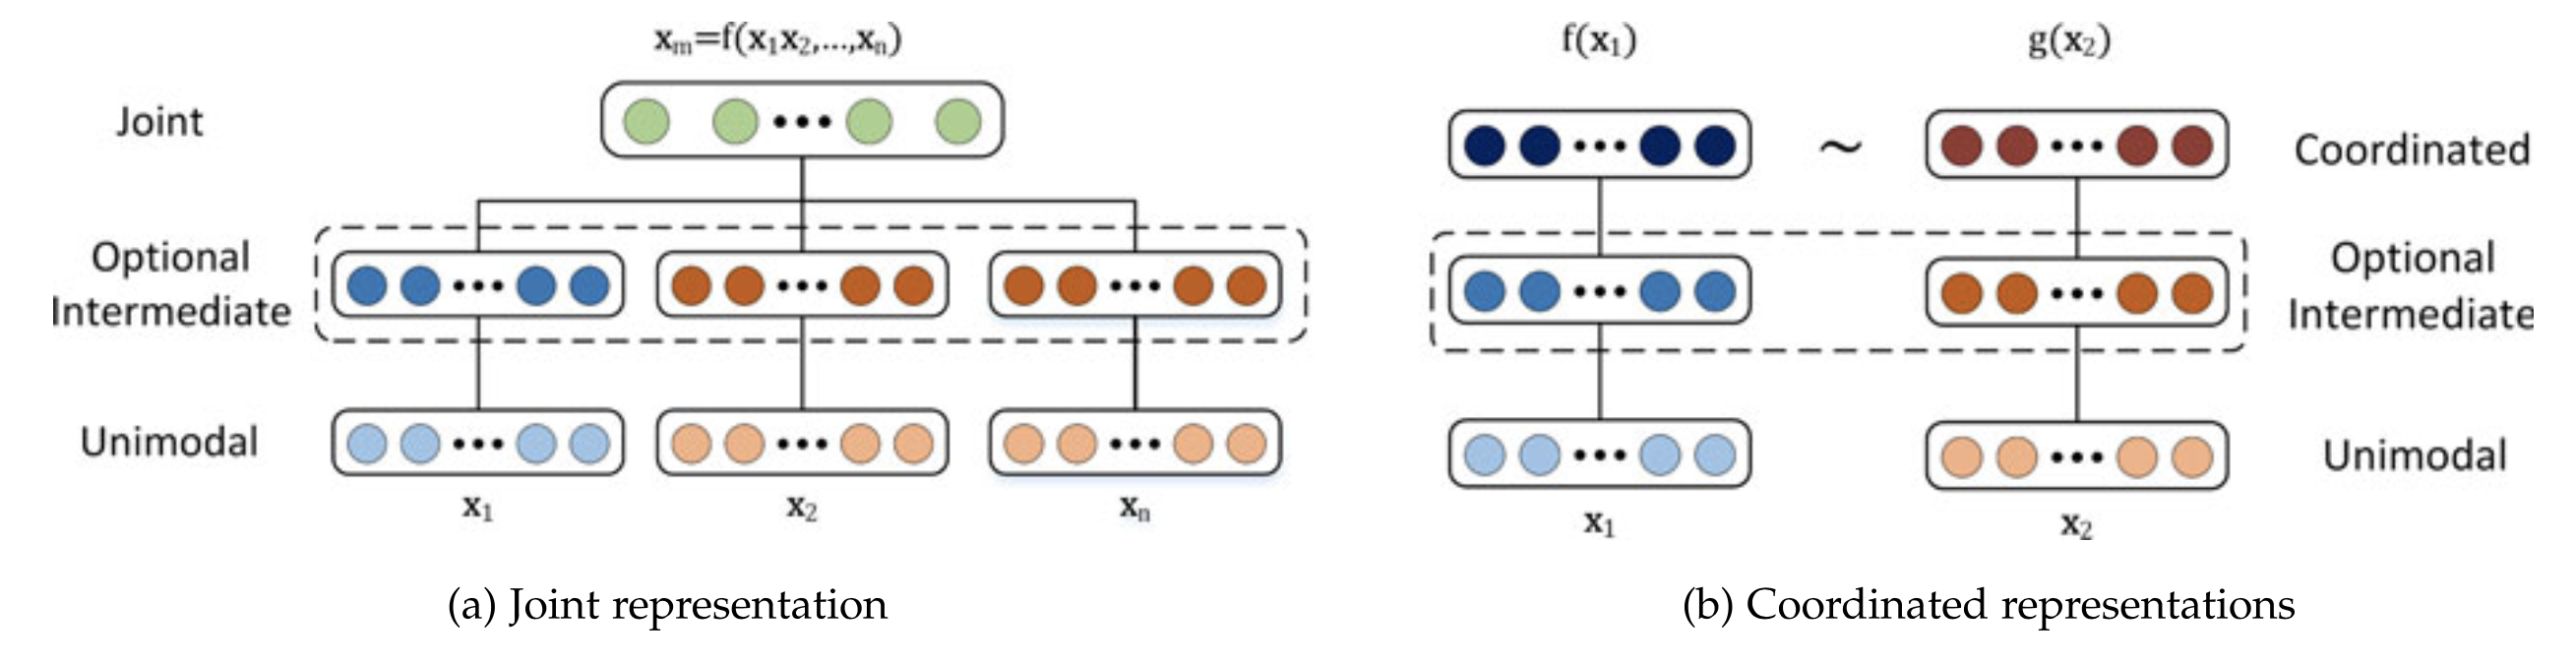
\includegraphics[width=0.95\textwidth,keepaspectratio]{images/2_literature/joint-vs-coordinated-representations.png}
\end{center}
\captionsetup{width=.90\textwidth}
\caption{Structure of joint and coordinated representation \cite{Baltrusaitis2017}}
\label{fig:structure-joint-coordinated}
\end{figure}

As mentioned before there hasn't been any research performed on multimodal fusion on road defects. In the broader sense, multimodal fusion has been applied to detect damages. Examples of which are: combining audio-visual data to detect conveyor belt damages \cite{Che2021}, gearbox fault detection based on vibrations and acoustic signals \cite{Li2016}. For more examples of applied data fusion in manufacturing industry, see \cite{Olivan2018}.

Further research shows that visual and accelerometer (IMU) data have been combined in odometry. With odometry the task is to estimate the location over time. For instance, calculating the current position, based on the previously known position. This is commonly applied in intelligent robots. Different motion sensors are fused to overcome ``dead-reckoning'', the loss of signal. Which can happen when the GPS data is lost or unstable \cite{Jiang2017,Brossard2020}.

One of the key challenges for this thesis is to synchronize the data sources. As mentioned earlier, this problem occurs because the camera sees an object on the road where the car will be driving after some delay. See also figure \ref{fig:synchronization}. Often in data fusion literature, modalities are misaligned due varying sampling rates, clock synchronization, or transmission delay between sensors. There are various known approaches to fix these issues. In general, the solution is designing a robust synchronization protocol to provide common notion of time. Existing methods often rely on a similarity measure or a trigger event between the different sources to fix this issue. Sensor synchronization is studied extensively in domain of sensor networks. When there is a similarity measure between the signals, the time delay between the signals can be calculated \cite{Liu2021}.


\begin{figure}[ht]
\begin{center}
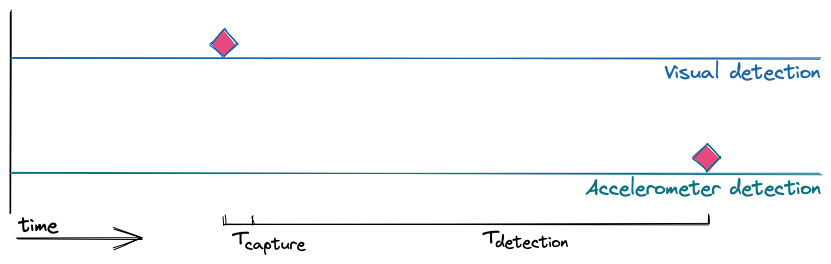
\includegraphics[width=0.95\textwidth,keepaspectratio]{images/2_literature/time-line-synchonization.png}
\end{center}
\captionsetup{width=.90\textwidth}
\caption{Illustration of the synchronization problem: there is a delay between detecting the object and driving over that object.}
\label{fig:synchronization}
\end{figure}


% To combine video and accelerometer data, the key operation is to find a similarity measure between both sources. From research we see this is done by estimating acceleration from video movement \cite{Fridman2015,Zhang2020}. Estimating of accelerations can be done using the dense optical flow algorithm. It is computed as a function of two frames taken at time $t$ and $t + \Delta t$, where $\Delta t$ depends on the frame rate. The method to calculate optical flow is as follows. First, an estimate for the velocity for every pixel in adjacent frames is computed using the Farneback algorithm \cite{Farnebäck2003}. The result is a 2D vector field, describing for each pixel the estimated motion in horizontal and vertical direction. By taking the average of all the estimated motions, a scalar acceleration is derived describing the acceleration of the frame.

% To synchronize the accelerometer data with the visual data, the time delay needs to be computed. Note, that in our case this calculated delay refers to the $\tau_{caputure}$, refer to section \ref{sec:relevance}. Cross correlation is a method often used to estimate the time delay between two signals \cite{Knapp1976}. Within the earlier research of \cite{Fridman2015, Zhang2020}, the authors also use cross correlation. Implementation of cross correlation is described in section \ref{sec:cross-correlation}.

% Another popular method for synchronization is Dynamic Time Warping (DTW). DTW measures the similarity between two sequences and finds the optimal match and inserts frames to align the time series. In our case we have a constant sampling frequency, thus using cross-correlation is sufficient, and is faster.


\subsection{Conclusion}
Automatic classification of road defects have been extensively researched. Main topic of interest is the usage of low-cost devices such as smartphones to collect the data. From the literature we find that only the following types of defects are classified: cracks, patches, holes and faded line markings. Other types of damages that are recognized by the CROW \cite{CROW_147}, but haven't been researched are raveling, rutting and skewed signs. Although this work doesn't try to classify those damages either, it illustrates an interesting gap in this field.

From our review, we conclude that there are some interesting papers to work from. First of all, we have the public data and models of the Road Damage Detector \cite{Arya2020-competition}. The authors frame the problem of detecting surface defects as object detection. This makes sense as damages in a image are basically objects. The best performing model uses the state-of-art model YOLOv5 \cite{rddc2020,Jocher2021}. During this work we'll also use YOLO to detect damages from visual data. As the authors describe in \authorref{Arya2020-transfer}, it unexpected that the pretrained model yields good results in a different country. By transfer learning the model on roads collected in the Netherlands, we improve the generalizability of the model.

Secondly, the research on detecting potholes using accelerometers uses a common methodology \cite{Wu2020,Basavaraju2019}. We'll also use this methodology, and apply the same processing steps of resampling, reorientation, and filtering. The implementation of these steps will be described later. 

Finally, we see that there hasn't been any research on multimodal machine learning in road defects detection. This makes this work novel, and an interesting contribution to the literature. From literature we learn that using neural networks is an easy method to implement multimodal machine learning \cite{Baltrusaitis2017}. 

